\documentclass[10pt,aspectratio=149]{beamer}

% All the boilerplate is in ac1slides.sty
% Note that this also pulls in a custom vogtwidebar.sty
\usepackage{ac1slides}

\author{Ji\v{r}\'i Lebl}

\institute[OSU]{%
Departemento pri Matematiko de Oklahoma {\^S}tata Universitato}

\title{BA: 5.1}

\date{}

\begin{document}

\begin{frame}
\titlepage
\end{frame}

\begin{frame}
An integral is a way to ``sum'' or ``average'' the values of a function.

\pause
\medskip

Integral is \emph{not} the antiderivative!

\pause
\medskip

An antiderivative can be computed via an integral,

\pause
but an integral does a lot more.

\pause
\medskip

In our setting, an integral is the ``area under the curve''

\pause
\medskip

We will follow the Darboux approach rather than Riemann approach,

they are equivalent.
\end{frame}

\begin{frame}

\begin{definition}
A \emph{partition} $P$ of the interval $[a,b]$ is
a finite set $\{ x_0,x_1,x_2,\ldots,x_n \}$ such that
\begin{equation*}
a = x_0 < x_1 < x_2 < \cdots < x_{n-1} < x_n = b .
\end{equation*}
\pause
We write
\begin{equation*}
\Delta x_i \coloneqq x_i - x_{i-1} .
\end{equation*}
\pause
Let $f \colon [a,b] \to \R$ be a bounded function.
\pause
Let $P$ be a partition of
$[a,b]$.
\pause
Define
\begin{align*}
& m_i \coloneqq \inf \, \bigl\{ f(x) : x_{i-1} \leq x \leq x_i \bigr\} , &
& M_i \coloneqq \sup \, \bigl\{ f(x) : x_{i-1} \leq x \leq x_i \bigr\} , \\
& L(P,f) \coloneqq
\sum_{i=1}^n m_i \Delta x_i , &
& U(P,f) \coloneqq
\sum_{i=1}^n M_i \Delta x_i .
\end{align*}
\pause
We call $L(P,f)$ the \emph{lower Darboux sum} and
$U(P,f)$ the \emph{upper Darboux sum}.
\end{definition}

\end{frame}

\begin{frame}

\begin{center}
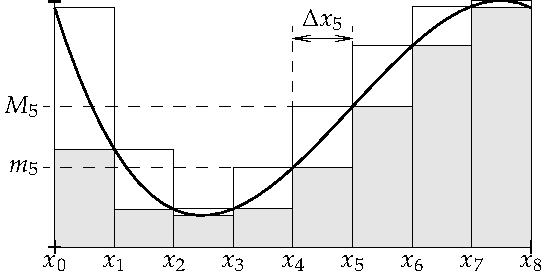
\includegraphics{../figures/darbouxfig}
\end{center}

\end{frame}

\begin{frame}

\begin{proposition}
Let $f \colon [a,b] \to \R$ be a bounded function.  Let $m, M \in \R$ be 
such that for all $x \in [a,b]$, we have $m \leq f(x) \leq M$.
\pause
Then for every partition $P$
of $[a,b]$,
\[
m(b-a) \leq
L(P,f) \leq U(P,f)
\leq M(b-a) .
\]
\end{proposition}

\pause
\textbf{Proof:}
Let $P$ be a partition of $[a,b]$.

\pause
$m \leq m_i$ for all $i$ and $M_i \leq M$ for all $i$.

\pause
$m_i \leq M_i$ for all $i$.

\pause
$\sum_{i=1}^n \Delta x_i = (b-a)$.

\pause
\medskip

\thus
\quad
$\displaystyle
m(b-a)
\pause
=
m \left( \sum_{i=1}^n \Delta x_i \right)
\pause
=
\sum_{i=1}^n m \Delta x_i
\pause
\leq
\sum_{i=1}^n m_i \Delta x_i 
$

\pause
\medskip

%There's an hfill in the qed
\hfill\hfill\hfill\hfill\hfill\hfill\hfill\hfill
\hfill\hfill\hfill\hfill\hfill\hfill\hfill\hfill
$\displaystyle
\leq
\sum_{i=1}^n M_i \Delta x_i
\pause
\leq
\sum_{i=1}^n M \Delta x_i 
\pause
=
M \left( \sum_{i=1}^n \Delta x_i \right)
\pause
=
M(b-a)
$.\qed

\pause
\medskip

In particular, the set of lower and
upper sums are bounded sets.
\end{frame}

\begin{frame}

\begin{definition}
As the sets of lower and upper Darboux sums are bounded, we define

\pause
\medskip

\qquad
$\displaystyle
\underline{\int_a^b} f(x)\,dx \coloneqq
\sup \, \bigl\{ L(P,f) : P \text{ a partition of } [a,b] \bigr\}$,

\pause
\bigskip

\qquad
$\displaystyle
\overline{\int_a^b} f(x)\,dx \coloneqq
\inf \, \bigl\{ U(P,f) : P \text{ a partition of } [a,b] \bigr\}$.

\pause
\medskip

We call $\underline{\int}$
the \emph{lower Darboux integral} and
$\overline{\int}$
the \emph{upper Darboux integral}.
\pause
To avoid worrying about the variable of integration, 
we often simply write
\begin{equation*}
\underline{\int_a^b} f \coloneqq
\underline{\int_a^b} f(x)\,dx 
\qquad \text{and} \qquad
\overline{\int_a^b} f \coloneqq
\overline{\int_a^b} f(x)\,dx  .
\end{equation*}
\end{definition}

\pause
\textbf{Remark:}
If $f \colon S \to \R$ and $[a,b] \subset S$,
use $f|_{[a,b]}$.  But we'll just write
$\underline{\int_a^b} f$ and
$\overline{\int_a^b} f$.

\end{frame}

\begin{frame}

\textbf{Example:}
Take the Dirichlet function
$f \colon [0,1] \to \R$, where $f(x) \coloneqq 1$ if
$x \in \Q$ and $f(x) \coloneqq 0$ if $x \notin \Q$.
\pause
Then
\begin{equation*}
\underline{\int_0^1} f = 0 \qquad \text{and} \qquad
\overline{\int_0^1} f = 1 .
\end{equation*}
\pause
Proof: Take any partition $P$.
\pause
For every $i$,

$m_i = \inf \bigl\{ f(x) : x \in [x_{i-1},x_i] \bigr\} = 0$~~
\pause
and
~~$M_i = \sup \bigl\{ f(x) : x \in [x_{i-1},x_i] \bigr\} = 1$.

\pause
\medskip

\thus \quad
$\displaystyle
L(P,f) = \sum_{i=1}^n 0 \cdot \Delta x_i = 0$,
\pause
\quad and \quad
$\displaystyle
U(P,f) = \sum_{i=1}^n 1 \cdot \Delta x_i = \sum_{i=1}^n \Delta x_i = 1$.
\qed

\end{frame}

\begin{frame}

\begin{definition}
Let $P = \{ x_0, x_1, \ldots, x_n \}$ and
$\widetilde{P} = \{ \widetilde{x}_0, \widetilde{x}_1, \ldots,
\widetilde{x}_{\ell} \}$ be
partitions of $[a,b]$.

\pause
We say $\widetilde{P}$ is a
\emph{refinement} of $P$
if as sets $P \subset \widetilde{P}$.
\end{definition}

\pause
\textbf{Example:}
$\{ 0, 0.5, 1, 2 \}$ is a partition of $[0,2]$

and
$\{ 0, 0.2, 0.5, 1, 1.5, 1.75, 2 \}$ is its refinement.

\pause
\medskip

\begin{proposition}
Let $f \colon [a,b] \to \R$ be bounded, $P$
a partition of $[a,b]$, $\widetilde{P}$ a refinement of $P$.
\pause
Then
\begin{equation*}
L(P,f) \leq L(\widetilde{P},f) 
\qquad \text{and} \qquad
U(\widetilde{P},f) \leq U(P,f) .
\end{equation*}
\end{proposition}

\end{frame}

\begin{frame}

\begin{proposition}
Let $f \colon [a,b] \to \R$ be bounded, $P$
a partition of $[a,b]$, $\widetilde{P}$ a refinement of $P$.
Then
\begin{equation*}
L(P,f) \leq L(\widetilde{P},f) 
\qquad \text{and} \qquad
U(\widetilde{P},f) \leq U(P,f) .
\end{equation*}
\end{proposition}

\pause
\textbf{Proof:}
Suppose $\widetilde{P} = \{ \widetilde{x}_0, \widetilde{x}_1, \ldots,
\widetilde{x}_{\ell} \}$ is
a refinement of 
$P = \{ x_0, x_1, \ldots, x_n \}$.

\pause
\thus \quad
$x_0 = \widetilde{x}_0$ and 
$x_n = \widetilde{x}_{\ell}$.

\pause
There are integers
$k_0 < k_1 < \cdots < k_n$ such that $x_i = \widetilde{x}_{k_i}$ for
$i=0,1,2,\ldots,n$.

\pause
Let
$\Delta x_i \coloneqq x_i - x_{i-1}$
and
$\Delta \widetilde{x}_q \coloneqq \widetilde{x}_q - \widetilde{x}_{q-1}$.

\pause
\medskip

\scalebox{0.8}{
\subimport*{../figures/}{figrefinement.pdf_t}
}

\pause
\medskip

$\displaystyle
\Delta x_i
\pause
=
x_i - x_{i-1}
\pause
=
\widetilde{x}_{k_i} - \widetilde{x}_{k_{i-1}}
\pause
=
\sum_{q=k_{i-1}+1}^{k_i} 
\widetilde{x}_{q} - \widetilde{x}_{q-1}
\pause
=
\sum_{q=k_{i-1}+1}^{k_i} \Delta \widetilde{x}_q
$.

\end{frame}

\begin{frame}

\scalebox{0.8}{
\subimport*{../figures/}{figrefinement.pdf_t}
}

\pause
\medskip

Let
$m_i \coloneqq \inf \bigl\{ f(x) : x_{i-1} \leq x \leq x_i \bigr\}$
and
$\widetilde{m}_q \coloneqq \inf \bigl\{ f(x) : \widetilde{x}_{q-1} \leq x \leq
\widetilde{x}_q \bigr\}$.

\pause
\medskip

$m_i \leq \widetilde{m}_q$ for $k_{i-1} < q \leq k_i$.

\pause
\medskip

\thus\quad
$\displaystyle
m_i \Delta x_i
\pause
=
m_i \sum_{q=k_{i-1}+1}^{k_i} \Delta \widetilde{x}_q
\pause
=
\sum_{q=k_{i-1}+1}^{k_i} m_i \Delta \widetilde{x}_q
\pause
\leq
\sum_{q=k_{i-1}+1}^{k_i} \widetilde{m}_q \Delta \widetilde{x}_q$.

\pause
\medskip

\thus\quad
$\displaystyle
L(P,f)
\pause
=
\sum_{i=1}^n m_i \Delta x_i
\pause
\leq
\sum_{i=1}^n \,
\sum_{q=k_{i-1}+1}^{k_i} \widetilde{m}_q \Delta \widetilde{x}_q
\pause
=
\sum_{q=1}^{\ell}
\widetilde{m}_q \Delta \widetilde{x}_q
\pause
= L(\widetilde{P},f)$.

\pause
\medskip

$U(\widetilde{P},f) \leq U(P,f)$ is left as an exercise.
\qed

\end{frame}

\begin{frame}

\begin{proposition}
Let $f \colon [a,b] \to \R$ be bounded.  Let $m, M \in \R$ be 
such that for all $x \in [a,b]$, we have $m \leq f(x) \leq M$.
\pause
Then
\vspace*{-12pt}
\[
m(b-a) \leq
\underline{\int_a^b} f \leq \overline{\int_a^b} f
\leq M(b-a) .
\]
\end{proposition}

\pause
\textbf{Proof:}
For any partition $P$, we proved \hfill
$m(b-a) \leq L(P,f) \leq U(P,f) \leq M(b-a)$.

\pause
\medskip

$m(b-a) \leq L(P,f)$ ~\thus~ $m(b-a) \leq \underline{\int_a^b} f$.
\pause
\quad
$U(P,f) \leq M(b-a)$ ~\thus~ $\overline{\int_a^b} f \leq M(b-a)$.

\pause
\medskip

%It's the middle inequality is the main idea.

Let $P_1, P_2$ be partitions of $[a,b]$.  Define $\widetilde{P} \coloneqq P_1 \cup P_2$.

\pause
$\widetilde{P}$ is a refinement of both $P_1$ and $P_2$

\pause
\thus
\quad
$L(P_1,f)
\pause
\leq L(\widetilde{P},f)
\pause
\leq U(\widetilde{P},f)
\pause
\leq U(P_2,f)$.

\pause
\medskip

\thus
\quad
$\underline{\int_a^b} f
\pause = 
\sup \, \bigl\{ L(P,f) : P \text{ a partition of } [a,b] \bigr\}
$

\pause
\qquad\qquad\qquad
$
\leq
\inf \, \bigl\{ U(P,f) : P \text{ a partition of } [a,b] \bigr\}
\pause
=
\overline{\int_a^b} f$.
\qed

\end{frame}

\begin{frame}

\begin{definition}
Let $f \colon [a,b] \to \R$ be bounded such that
\begin{equation*}
\underline{\int_a^b} f(x)\,dx = \overline{\int_a^b} f(x)\,dx .
\end{equation*}
\pause
Then $f$ is said to be \emph{Riemann integrable}.
\pause
The set of Riemann integrable functions on $[a,b]$ is denoted
by $\sR[a,b]$.
\pause
When $f \in \sR[a,b]$, we define
\begin{equation*}
\int_a^b f(x)\,dx \coloneqq 
\underline{\int_a^b} f(x)\,dx = \overline{\int_a^b} f(x)\,dx .
\end{equation*}
\pause
We often write
\begin{equation*}
\int_a^b f \coloneqq \int_a^b f(x)\,dx.
\end{equation*}
\pause
$\int_a^b f$ is called the \emph{Riemann integral}
of $f$, or simply the \emph{integral} of $f$.
\end{definition}

\end{frame}

\begin{frame}

We immediately get:

\begin{proposition}
Let $f \colon [a,b] \to \R$ be Riemann integrable.
Let $m, M \in \R$ be 
such that $m \leq f(x) \leq M$ for all $x \in [a,b]$.  Then
\vspace*{-12pt}
\begin{equation*}
m(b-a) \leq
\int_a^b f
\leq M(b-a) .
\end{equation*}
\end{proposition}

\pause

\begin{center}
\scalebox{0.8}{
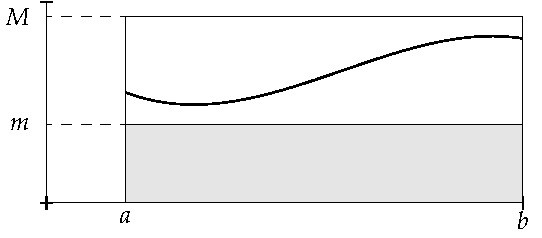
\includegraphics{../figures/integralminmax}
}
\end{center}

\pause
Useful version:
If $\abs{f(x)} \leq M$ for all $x \in [a,b]$, then
\quad
$\displaystyle
\bbabs{\int_a^b f} \leq M(b-a)$.

\end{frame}

\begin{frame}

\textbf{Example:}
Constant function are integrable:

\pause
\medskip

If $f(x) =c$ for some constant $c$, then $c$ is an upper and lower bound,
\pause
so
\[
c(b-a) \leq
\underline{\int_a^b} f \leq \overline{\int_a^b} f
\leq c(b-a) .
\]

\pause
So $f$ is integrable on any interval $[a,b]$ and
\[
\int_a^b f = c(b-a) .
\]

\end{frame}

\begin{frame}

\textbf{Example:}
Let $f \colon [0,2] \to \R$ be defined by
\begin{equation*}
f(x) \coloneqq
\begin{cases}
1               & \text{if } x < 1,\\
\nicefrac{1}{2} & \text{if } x = 1,\\
0               & \text{if } x > 1.
\end{cases}
\end{equation*}
\pause
We claim $f$ is Riemann integrable and $\displaystyle \int_0^2 f = 1$.

\pause
\medskip

Proof: Let $0 < \epsilon < 1$ be arbitrary.

\pause
Let $P \coloneqq \{0, 1-\epsilon, 1+\epsilon, 2\}$ be a partition.

\pause
Using the notation from before:
\begin{align*}
m_1 &= \inf \, \bigl\{ f(x) : x \in [0,1-\epsilon] \bigr\} = 1 , & 
M_1 &= \sup \, \bigl\{ f(x) : x \in [0,1-\epsilon] \bigr\} = 1 , \\
m_2 &= \inf \, \bigl\{ f(x) : x \in [1-\epsilon,1+\epsilon] \bigr\} = 0 , & 
M_2 &= \sup \, \bigl\{ f(x) : x \in [1-\epsilon,1+\epsilon] \bigr\} = 1 , \\
m_3 &= \inf \, \bigl\{ f(x) : x \in [1+\epsilon,2] \bigr\} = 0 , & 
M_3 &= \sup \, \bigl\{ f(x) : x \in [1+\epsilon,2] \bigr\} = 0 .
\end{align*}
\pause
Furthermore, ~~$\Delta x_1 = 1-\epsilon$,
~~$\Delta x_2 = 2\epsilon$,~~ and ~~$\Delta x_3 = 1-\epsilon$.

\end{frame}

\begin{frame}

\begin{center}
\scalebox{0.8}{
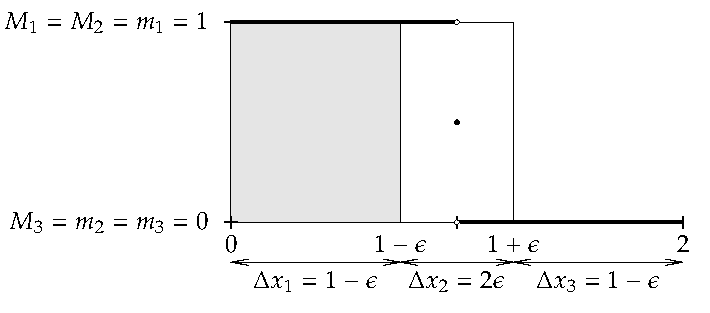
\includegraphics{../figures/darbouxfigstep}
}
\end{center}

\pause
\medskip

$\displaystyle
L(P,f)
\pause
= \sum_{i=1}^3 m_i \Delta x_i
\pause
=
1 \cdot (1-\epsilon) + 0 \cdot 2\epsilon + 0 \cdot (1-\epsilon)
\pause
= 1-\epsilon$,

\pause
\medskip

$\displaystyle
U(P,f)
\pause
= \sum_{i=1}^3 M_i \Delta x_i
\pause
=
1 \cdot (1-\epsilon) + 1 \cdot 2\epsilon + 0 \cdot (1-\epsilon)
\pause
= 1+\epsilon$.

\pause
\medskip

\thus\quad
$\displaystyle
\overline{\int_0^2} f - 
\underline{\int_0^2} f
\pause
\leq
U(P,f) - L(P,f)
\pause
=
(1+\epsilon)
- (1-\epsilon) = 2 \epsilon$.

\end{frame}

\begin{frame}
$\displaystyle \overline{\int_0^2} f - \underline{\int_0^2} f \leq 2 \epsilon$
\qquad
\pause
also
\qquad
$\displaystyle \underline{\int_0^2} f \leq \overline{\int_0^2} f$

\pause
\medskip

As $\epsilon$
was arbitrary
\pause
\wthus
$\displaystyle \overline{\int_0^2} f = \underline{\int_0^2} f$
\pause
\wthus
 $f$ is Riemann integrable.

\pause
\bigskip

$\displaystyle
1-\epsilon
\pause
= L(P,f)
\pause
\leq \int_0^2 f
\pause
\leq U(P,f)
\pause
=
1+\epsilon$
\pause
\wthus
$\displaystyle\bbabs{\int_0^2 f - 1 } \leq \epsilon$.

\pause
\medskip

As $\epsilon$ was arbitrary
\pause
\wthus
$\displaystyle \int_0^2 f = 1$.
\qed

\end{frame}

\begin{frame}

\begin{proposition}
Let $f \colon [a,b] \to \R$ be bounded.  Then $f$ is Riemann
integrable if for every $\epsilon > 0$, there exists a partition $P$ of
$[a,b]$ such that
\begin{equation*}
U(P,f) - L(P,f) < \epsilon .
\end{equation*}
\end{proposition}

\pause
\textbf{Proof:}
If for every $\epsilon > 0$ such a $P$ exists, then
\begin{equation*}
0 \leq
\overline{\int_a^b} f - 
\underline{\int_a^b} f
\pause
\leq
U(P,f) - L(P,f)
\pause
< \epsilon .
\end{equation*}
\pause
\thus \quad
$\displaystyle \overline{\int_a^b} f = \underline{\int_a^b} f$
\pause
\wthus
$f$ is integrable.
\qed

\end{frame}

\begin{frame}

\textbf{Example:}
Claim: $\frac{1}{1+x}$ is integrable on $[0,b]$ for any $b > 0$.

\pause
\medskip

Proof: Let $\epsilon > 0$ be given.

\pause
Take $n \in \N$ and
\pause
let $x_i \coloneqq \nicefrac{ib}{n}$,
\pause
to get partition
$P \coloneqq \{ x_0,x_1,\ldots,x_n \}$ of $[0,b]$.

\pause
$\Delta x_i = \nicefrac{b}{n}$ for all $i$.  

\pause
\medskip

$f$ is decreasing so
$
m_i = \inf \left\{ \frac{1}{1+x} : x \in [x_{i-1},x_i] \right\} =
\frac{1}{1+x_i}$,

\pause
and
$M_i = \sup \left\{ \frac{1}{1+x} : x \in [x_{i-1},x_i] \right\} =
\frac{1}{1+x_{i-1}}$.

\pause
\medskip

\thus \quad
$\displaystyle
U(P,f)-L(P,f)
\pause
=
\sum_{i=1}^n
\Delta x_i
(M_i-m_i)
\pause
=
\frac{b}{n}
\sum_{i=1}^n 
\left( \frac{1}{1+\nicefrac{(i-1)b}{n}} - \frac{1}{1+\nicefrac{ib}{n}} \right) 
$

\pause
\medskip

\qquad\qquad\qquad
$\displaystyle
=
\frac{b}{n}
\left( \frac{1}{1+\nicefrac{0b}{n}} - \frac{1}{1+\nicefrac{nb}{n}} \right) 
\pause
=
\frac{b^2}{n(b+1)}$.

\pause
\medskip

Pick $n$ to be such that
$\frac{b^2}{n(b+1)} < \epsilon$,
\pause
the proposition is satisfied,

\pause
and the function is integrable.
\end{frame}

\begin{frame}

\textbf{Remark:}
The integral adds up (integrates) local information---it sums $f(x)\,dx$ over all $x$.

\pause
\medskip

Derivatives are ``local'', only ``at a point'':

velocity, acceleration, rate of change,
slope \ldots

\pause
\medskip

Integrals are ``global'':

total distance travelled, average temperature,
total charge \ldots

\pause
\medskip

\textbf{Notation:}
If $f \colon S \to \R$ and $[a,b] \subset S$,
use the restriction, but write $\int_a^b f$ and $f \in \sR[a,b]$.

\pause
\medskip

We define $\int_a^b f$ even if $a \not< b$:

\pause
\medskip

If $b < a$ and $f \in \sR[b,a]$,
then define
\quad
$\displaystyle
\int_a^b f \coloneqq - \int_b^a f$.
\quad
\pause
Also
\quad
$\displaystyle
\int_a^a f \coloneqq 0$.

\pause
\medskip

The $x$ in $dx$ is just a dummy variable,
so, e.g.,
\quad
$\displaystyle
\int_a^b f(s)\,ds \coloneqq \int_a^b f(x)\,dx$.

\end{frame}

\begin{frame}

\textbf{Remark:}
Here's the Riemann approach to integrating
$f \colon [a,b] \to \R$.

\pause
Take a partition
$P = \{ x_0, x_1, \ldots, x_n \}$

\pause
and a set of numbers (tags) $\{ c_1, c_2, \ldots, c_n \}$ with
$c_k \in [x_{k-1},x_k]$ for all $k$.

\pause
Then compute the \emph{Riemann sum}:
\quad
$\displaystyle
\sum_{k=1}^n f(c_k) \Delta x_k$.

\pause
\medskip

The normal definition of Riemann integrable is if a number $I$
exists such that for every $\epsilon > 0$ there exists a
$\delta > 0$ such that if $P$ is a partition with $\Delta x_i < \delta$
for all $i$, then for any set of tags,
the Riemann sum is within $\epsilon$ of $I$.

\pause
\medskip

\textbf{Exercise:}
Prove that if $f$ is Riemann integrable, then for any $\epsilon > 0$
there exists a Riemann sum that is within $\epsilon$ of the integral.

\end{frame}

\end{document}
